\section{Definierung der Skill-Struktur} \label{Skillstruktur}
	Alle Skills sollten nach einer einheitlichen Struktur aufgebaut sein und lediglich um die prozessspezifischen Funktionen ergänzt werden. Ein zentraler Bestandteil dieser Grundstruktur sind die Schnittstellen, die ein Skill mindestens benötigt, um innerhalb der Systemstruktur funktionsfähig zu sein. Dazu zählen nicht nur Eingangs- und Ausgangsvariablen, sondern auch Eigenschaften und Methoden, da Informationen ebenfalls über diese übertragen werden können. Ein Skill muss über die definierten Schnittstellen (siehe Kapitel \ref{Softwareinteraktion}) sowohl mit dem System, mit dem Objekt und innerhalb des Prozessmodells interagieren können. 
	\\
	Innerhalb der Entwicklung wurden mehrere Iterationen von Skill-Strukturen geplant, umgesetzt und getestet, um die bestmöglichste Struktur zu finden. Innerhalb dieser Dokumentation werden nicht alle Iterationsschritte erklärt, sondern nur die daraus folgenden Erkenntnisse. 
	\\
	Die Schnittstellen eines Skills wurden in drei Kategorien aufgeteilt, welche das allgemeine Verständnis einfacher machen sollen.
	
	\textbf{Steuerungselemente:}
	\vspace{2mm} 
	\\
	Die Steuerungselemente sind für die Bedienung des Skills angedacht. Hier wird der Skill gestartet, gestoppt oder resettet. Zusätzlich werden auch Informationen über den Zustand des Skills angegeben.
	
	\textbf{Betriebselemente:}
	\vspace{2mm} 
	\\
	Die Betriebselemente sind für den allgemeinen Betrieb des Skills angedacht, welche nicht mit dem spezifischen Prozess zu tun haben. Dies ist zum Beispiel die Schnittstelle zum System, welche eine Aussage über Systemzustand macht. 
	
	\textbf{Prozesselemente:}
	\vspace{2mm} 
	\\
	Die Prozesselemente sind spezifische Informationen, welche der Skill für die Ausführung benötigt und dann auch an das Objekt weitergibt. 
	
	Zu Beginn wurden die Steuerungselemente auf Basis des PLC-Standards aufgebaut. Der Skill wurde dabei von einer BOOL-Variable (bExecute) gestartet und hat diverse Informationen als Ausgangsvariablen ausgegeben (bDone, bBusy, bLimit, bError und iErrorID). Die Ausgangsvariablen konnten als Transition-Bedingungen für Abläufe verwendet werden. Auf den ersten Blick ist dies eine einfache und sinnvolle Steuerung des Skills. Jedoch zeigte sich bei ersten Versuchen, dass diese Implementierung diverse Probleme mit sich bringen kann. Die Umsetzung eines bExecute-Triggers ist aufwändig und muss gut durchdacht werden, da der Skill nur einmal ausgeführt werden soll. Wenn der Skill beendet wurde und die bExecute-Variable immer noch betätigt ist, soll der Skill nicht ein zweites Mal gestartet werden. Der Trigger muss entsprechend so umgesetzt werden, dass dieser nur auf eine steigende Flanke reagiert. Das Management der Ausgangsvariablen ist geknüpft an die verschiedenen Zustände innerhalb des Skills. Es muss genau bestimmt werden, welcher Zustand einen Einfluss auf die Ausgänge hat. Durch die hohe Anzahl an Ausgangsvariablen, kann man hierbei schnell den Überblick verlieren. Zusätzlich werden viele der Informationen, welche über die Ausgangsvariablen dargestellt werden, auch über den Zustand dargestellt werden. Die Konsequenz daraus ist, dass die Steuerungselemente mit Methoden und Eigenschaften umgesetzt werden (\ref{tab:Skill_Steuerungselemente}). 
	
	\newpage
	
	\begin{table}[ht]
		\centering
		\colorlet{BFH-table}{BFH-MediumBlue!10}
		\colorlet{BFH-tablehead}{BFH-MediumBlue!50}
		\begin{bfhTabular}{clcl}
			Art: 		& Bezeichnung:		& Typ:		& Beschreibung:								
			\\\hline
			Methode		& \verb|M_Start|		& BOOL			& Methode zum Starten des Skills
			\\\hline
			Methode		& \verb|M_Stop|			& BOOL			& Methode zum Stoppen des Skills
			\\\hline
			Methode		& \verb|M_Reset|		& BOOL			& Methode zum Resetten des Skills
			\\\hline
			Eigenschaft	& \verb|P_State|	& eSkillState		& Eigenschaft des aktuellen Zustandes
		\end{bfhTabular}
		\captionsetup{justification=centering}
		\caption{Steuerungselemente eines Skills}
		\label{tab:Skill_Steuerungselemente}
	\end{table}
	
	 Die Eigenschaft wird mit einem benutzerdefinierten Datentyp umgesetzt (\ref{tab:eSkillState}), welche die Zustände des Skills abbildet. Somit ist immer klar, in welchem Zustand sich der Skill im Moment befindet. 
	 
	 \begin{table}[ht]
	 	\centering
	 	\colorlet{BFH-table}{BFH-MediumBlue!10}
	 	\colorlet{BFH-tablehead}{BFH-MediumBlue!50}
	 	\begin{bfhTabular}{cc}
	 		Listen-Nr: 		& eSkillState:									
	 		\\\hline
	 		0				& \verb|BEREIT|	
	 		\\\hline
	 		1				& \verb|LAUFEND|		
	 		\\\hline
	 		2				& \verb|ABGESCHLOSSEN|		
	 		\\\hline
	 		3				& \verb|FEHLER|	
	 		\\\hline
	 		4				& \verb|LIMIT|	
	 		\\\hline
	 		5				& \verb|ERREICHT|	
	 	\end{bfhTabular}
	 	\captionsetup{justification=centering}
	 	\caption{Definition von eSkillState}
	 	\label{tab:eSkillState}
	 \end{table}
	 
	 Auch bei den Betriebselementen gab es im Verlauf der Entwicklung Veränderungen. Zu Beginn enthielten diese alle Variablen, die für den Betrieb des Skills erforderlich waren, und dienten als Schnittstelle zwischen System und Objekt. Relevante Informationen für den Prozess wurden dabei über Ausgangsvariablen an das Objekt übergeben, welches diese wiederum als Eingangsvariablen entgegennahm.
	 \\
	 Wenn jedoch zwei Skills auf dasselbe Objekt zugreifen sollen (nicht gleichzeitig) und beide mit dessen Eingangsvariablen verbunden sind, überschreibt stets einer der beiden Skills den Wert des anderen. Da es durchaus vorkommt, dass mehrere Skills mit einem Objekt interagieren (ebenfalls nicht gleichzeitig), muss die Interaktion zwischen Skill und Objekt so gestaltet sein, dass sie unabhängig von anderen Skills funktioniert.
	 \\
	 \begin{wrapfigure}{r}{0.45\textwidth}
	 	\centering
	 	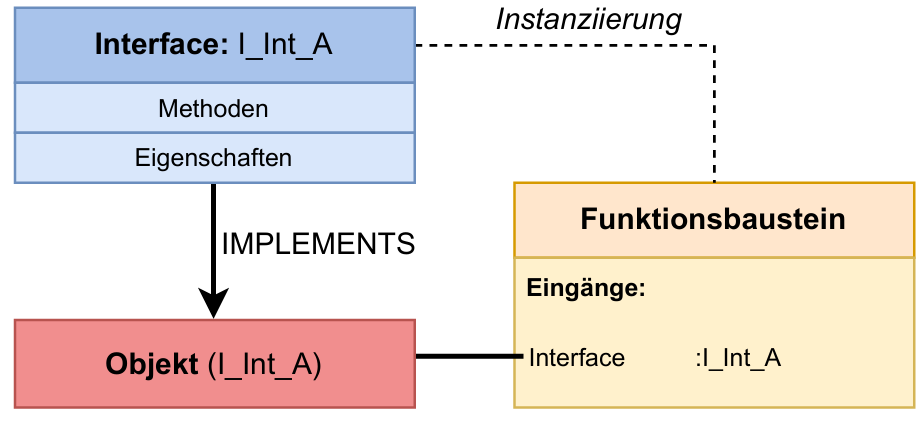
\includegraphics[width=0.45\textwidth]{06_Skillentwicklung/Schnittstellenstruktur}
	 	\captionsetup{justification=centering}
	 	\caption{Schnittstellenstruktur}
	 	\label{fig:Schnittstellenstruktur}
	 \end{wrapfigure} Dies lässt sich durch die Instanziierung eines Interfaces erreichen. In der objektorientierten Programmierung wird ein Interface genutzt, um vorzugeben, welche Methoden und Eigenschaften ein Funktionsbaustein zwingend besitzen muss. Durch das Instanziieren eines Interfaces innerhalb eines Funktionsbausteins können dessen Methoden und Eigenschaften verwendet werden. Wenn eine Eingangsvariable mittels Interface instanziiert wird, kann diese Funktionsbaustein-Eingangsvariable mit einem Objekt verbunden werden, insofern das selbe Interface beim Objekt implementiert wurde (\ref{fig:Schnittstellenstruktur}). Beim Ausführen einer Methode innerhalb des Funktionsbausteins wird dadurch die entsprechende Methode im verknüpften Objekt aufgerufen. Gleiches gilt für die Eigenschaften. Dadurch kann z.B. der Zustand des Objektes über diese Schnittstelle abgefragt werden. 
	 
	 \newpage
	 
	 Somit wurden die Betriebselemente wie folgt definiert: 
	 
	 \begin{table}[ht]
	 	\centering
	 	\colorlet{BFH-table}{BFH-MediumBlue!10}
	 	\colorlet{BFH-tablehead}{BFH-MediumBlue!50}
	 	\begin{bfhTabular}{clcl}
	 		Art: 				& Bezeichnung:			& Typ:				& Beschreibung:								
	 		\\\hline
	 		Eingangsvariabel	& \verb|eSysCommand|	& eSystemCommand	& Befehl von System zu Skill
	 		\\\hline
	 		Eingangsvariabel	& \verb|eSysState|		& eSystemStatus		& Informationen über System 
	 		\\\hline
	 		Eingangsvariabel	& \verb|fbObjekt|		& Objekt Interface	& Verknüpfung zu Objekt
	 		\\\hline
	 		Ausgangsvariabel	& \verb|iErrorID|		& INT				& Information über Fehler
	 	\end{bfhTabular}
	 	\caption{Betriebselemente eines Skills}
	 	\label{tab:Skill_Betriebselemente}
	 \end{table}
	 
	 Da auch die Übergabe der Objektparameter an das Objekt über die Interface-Verknüpfung erfolgt (mittels einer Eigenschaft), wird für jede Art von Objekttyp ein eigenes Interface definiert. Die Steuerungselemente für ein Objekt sind jedoch für alle Objekttypen einheitlich und ähnlich wie bei den Skills. Dazu gehören die Methoden \verb|M_Start|, \verb|M_Stop|, \verb|M_Rest| sowie die Eigenschaft \verb|P_State| (ObjectState).
	 \\
	 Die folgenden benutzerdefinierten Datentypen sind für die Betriebselemente von Bedeutung:
	 
	  \begin{table}[ht]
	 	\centering
	 	\colorlet{BFH-table}{BFH-MediumBlue!10}
	 	\colorlet{BFH-tablehead}{BFH-MediumBlue!50}
	 	\begin{bfhTabular}{cccc}
	 		Listen-Nr: 	& eSystemCommand:	& ObjectState:	& eSystemState:									
	 		\\\hline
	 		0			& \verb|KEINE|		& \verb|AUS|					& \verb|AUS| 
	 		\\\hline
	 		1			& \verb|AUSSCHALTEN|& \verb|BEREIT|					& \verb|BEREIT|
	 		\\\hline
	 		2			& \verb|EINSCHALTEN|& \verb|MANUELL|				& \verb|LAUFEND|
	 		\\\hline
	 		3			& \verb|STOPPEN|	& \verb|LAUFEND|				& \verb|GESTOPPT|
	 		\\\hline
	 		4			& \verb|RESETTEN|	& \verb|ABGESCHLOSSEN_INTERN|	& \verb|FEHLER|
	 		\\\hline
	 		5			& \verb|/|			& \verb|ABGESCHLOSSEN_EXTERN|	& \verb|/|
	 		\\\hline
	 		6			& \verb|/|			& \verb|GESTOPPT|				& \verb|/|
	 		\\\hline
	 		7			& \verb|/|			& \verb|FEHLER|					& \verb|/|
	 	\end{bfhTabular}
	 	\captionsetup{justification=centering}
	 	\caption{Benutzerdefinierte Datentypen}
	 	\label{tab:Datentypen_Benutzerdefiniert}
	 \end{table}
	 
	 \begin{bfhNoteBox}
	 	Beim Datentyp \verb|"ObjectState"| wird unterschieden zwischen einem Aktor oder einem Sensor. Die dargestellten Zustände beziehen sich auf einen Aktor. Innerhalb von Kaptiel \ref{Entwicklung des Anlagenmodells} wird detaillierter auf den Unterschied zwischen Aktoren und Sensoren eingegangen. 
	 \end{bfhNoteBox}
	 \vspace{3mm}
	 
	 Als letzte Kategorie umfasst die Prozesselemente. Die Prozesseigenschaften dienen dem bereitstellen von prozessrelevanten Informationen. Die vorhandenen Prozessmethoden werden vom Skill intern genutzt, beispielsweise zur Datenverarbeitung oder  Auswertung.
	 \\
	 Ähnlich wie bei einem Objekt wird auch ein Skill mithilfe eines Interfaces aufgebaut, das die zugehörigen Methoden und Eigenschaften definiert. Über die Interface-Verknüpfung lässt sich ein Skill zudem einfach in eine Sequenz oder einen Arbeitsplan integrieren.
	 
	 \newpage
	 
	 Die Grundstruktur eines Skills lässt sich anhand des folgenden Schemas zusammenfassen (\ref{fig:Skillschnittstellen}). Dieses Schema veranschaulicht auch die Interaktion des Skills über die verschiedenen Schnittstellen im System.
	 
	 \begin{figure}[h!]
	 	\centering
	 	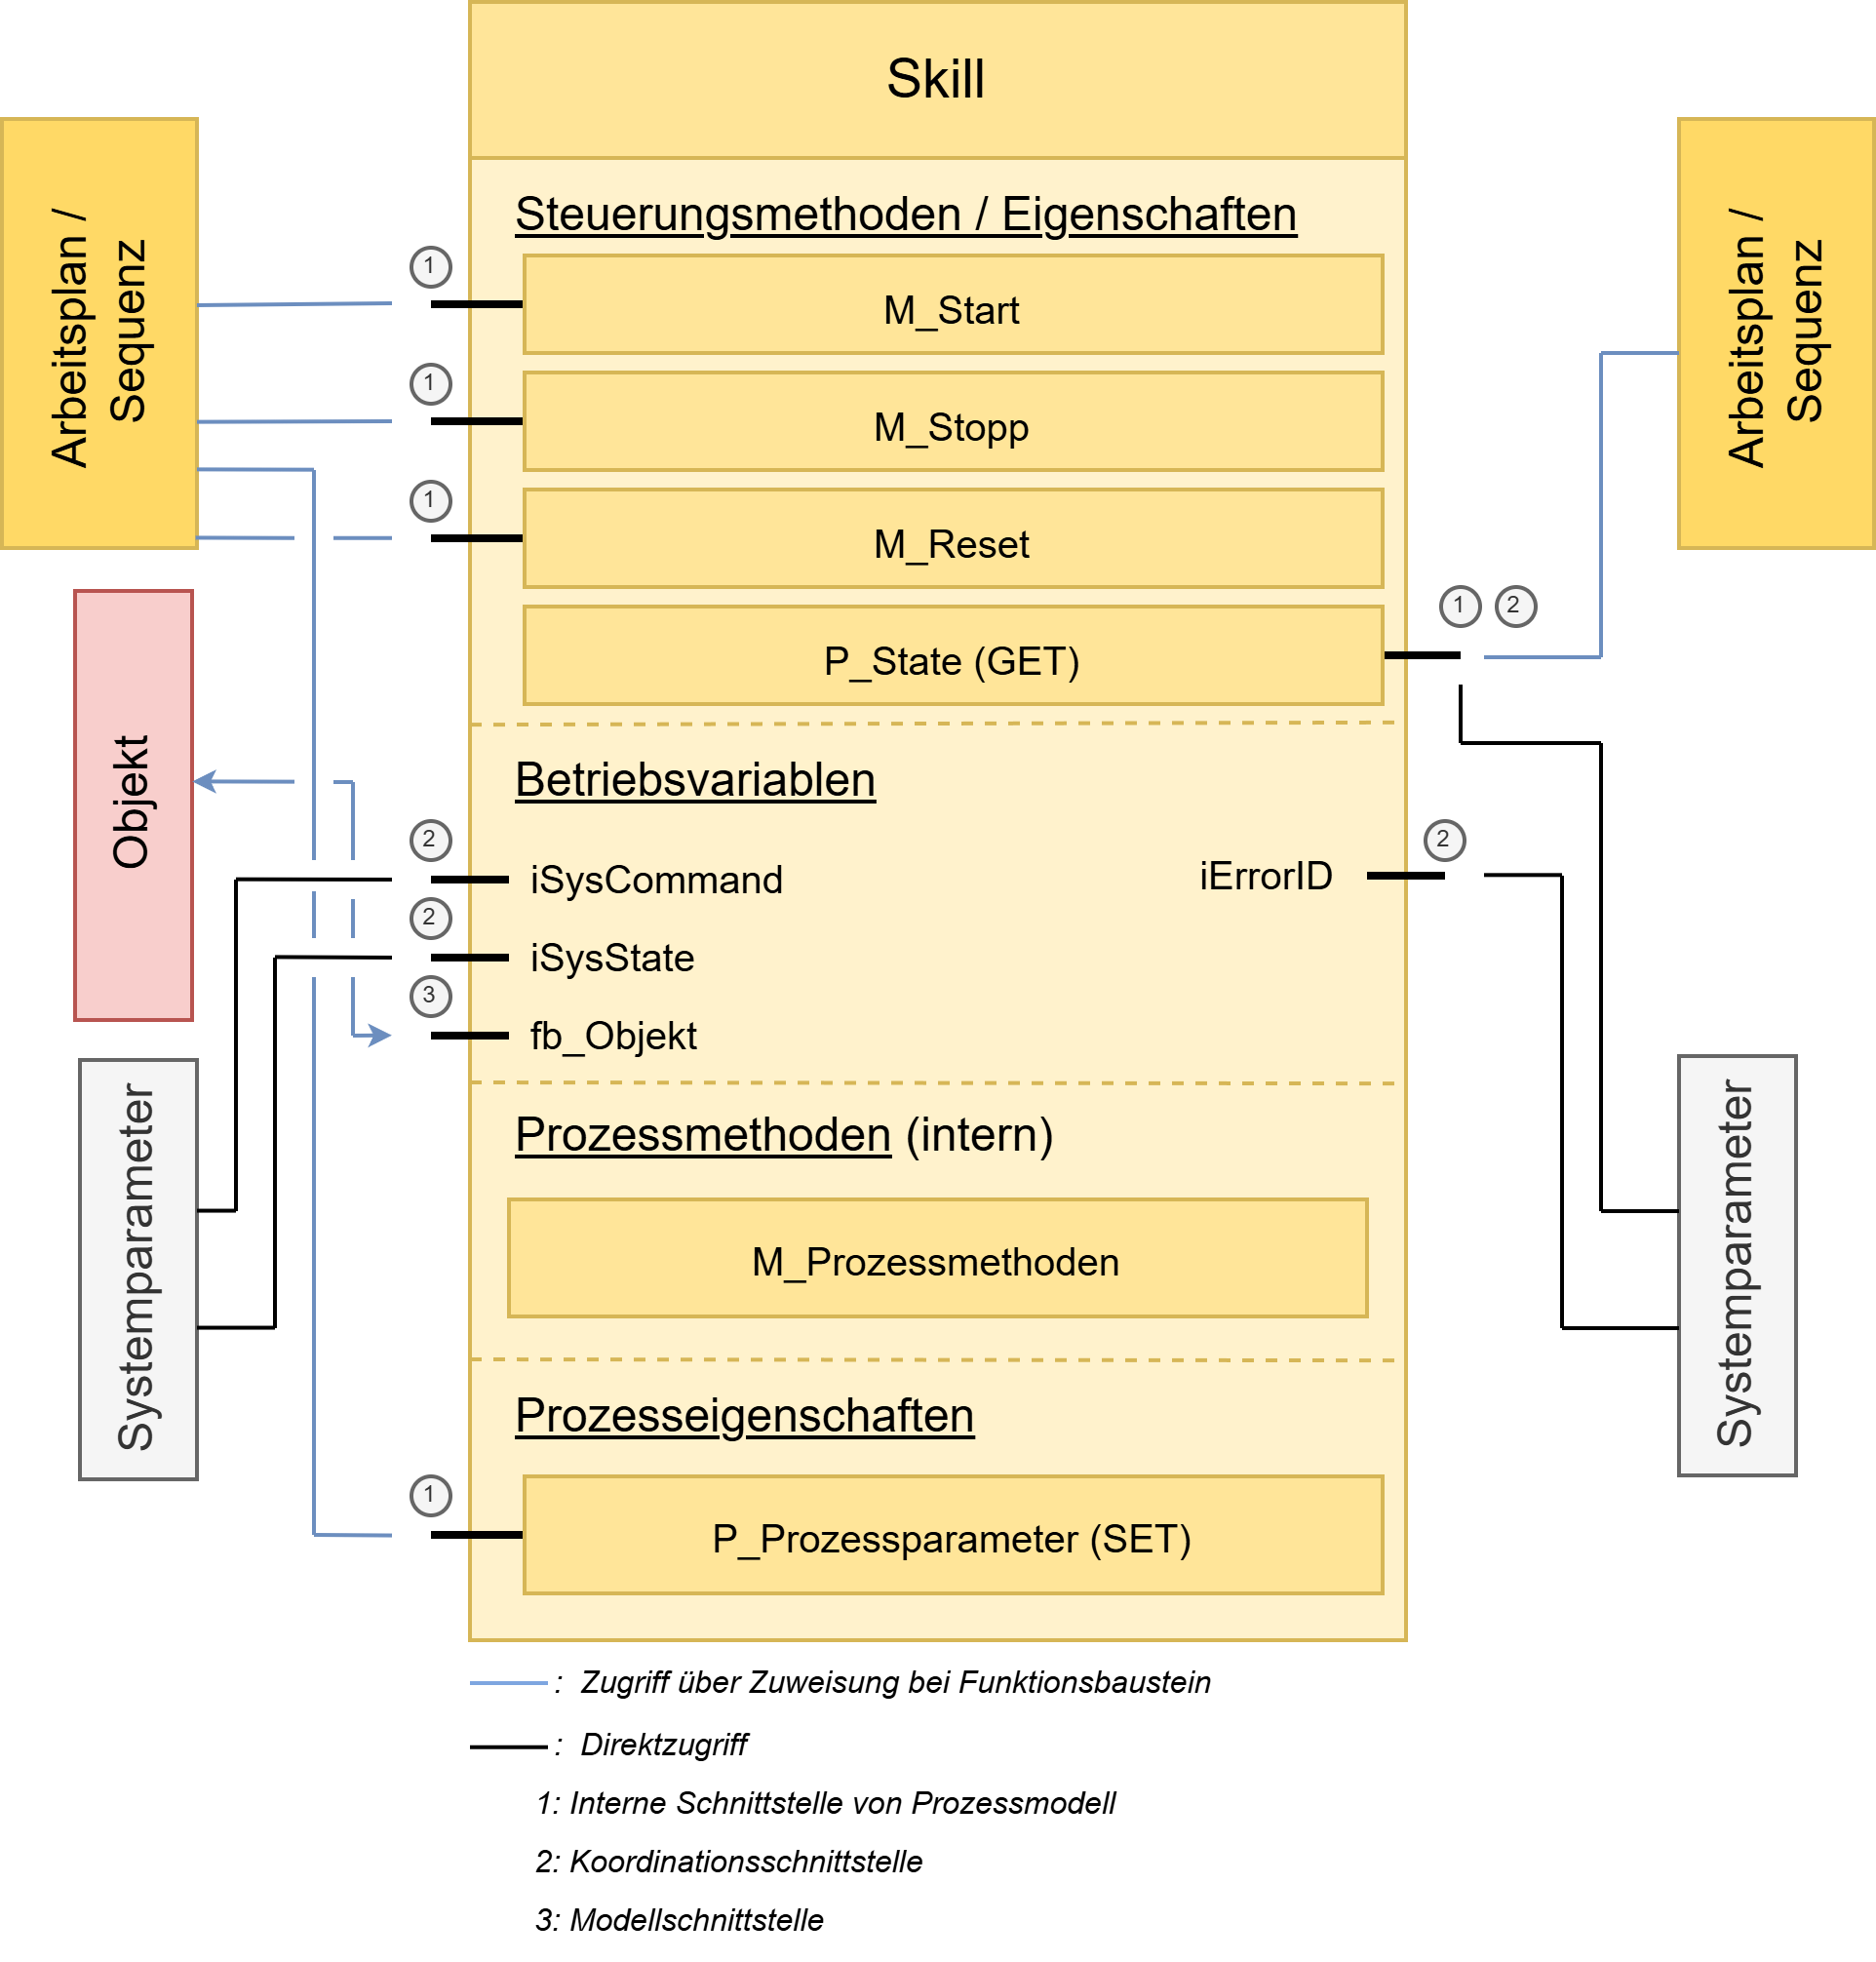
\includegraphics[width=0.9\textwidth]{06_Skillentwicklung/Skillschnittstellen}
	 	\captionsetup{justification=centering}
	 	\caption{Skilldefinition und Schnittstellen}
	 	\label{fig:Skillschnittstellen}
	 \end{figure}
	 
	 \newpage
	 
	 